\documentclass[conference,compsoc]{IEEEtran}

% *** CITATION PACKAGES ***
%
\ifCLASSOPTIONcompsoc
  % IEEE Computer Society needs nocompress option
  % requires cite.sty v4.0 or later (November 2003)
  \usepackage[nocompress]{cite}
\else
  % normal IEEE
  \usepackage{cite}
\fi

% *** GRAPHICS RELATED PACKAGES ***
%
\ifCLASSINFOpdf
\else
\fi

% correct bad hyphenation here
\hyphenation{op-tical net-works semi-conduc-tor}
\usepackage{amssymb} %mathematical packages to write correct' formulas
\usepackage{amsmath}
\usepackage{graphicx}
\usepackage{float}

\begin{document}

\title{Optimizing the loading of a truck in order\\
to make best use of space\\
and increase revenue a single transport }


% author names and affiliations
% use a multiple column layout for up to three different
% affiliations
\author{
\IEEEauthorblockN{Lukasz Joksch}
\IEEEauthorblockA{Department of Electronics,\\Wroclaw University of Technology\\Wroclaw, Poland\\
E-mail:lukaszjok@gmail.com}
\and
\IEEEauthorblockN{Tomasz Kowalik}
\IEEEauthorblockA{Department of Electronics,\\Wroclaw University of Technology\\Wroclaw, Poland\\
tomasz\_kowalik@hotmail.com}
\and
\IEEEauthorblockN{Piotr Tazbir}
\IEEEauthorblockA{Department of Electronics,\\Wroclaw University of Technology\\Wroclaw, Poland\\
E-mail: piter9901@gmail.com }
}

% conference papers do not typically use \thanks and this command
% is locked out in conference mode. If really needed, such as for
% the acknowledgment of grants, issue a \IEEEoverridecommandlockouts
% after \documentclass

% for over three affiliations, or if they all won't fit within the width
% of the page (and note that there is less available width in this regard for
% compsoc conferences compared to traditional conferences), use this
% alternative format:
% 
%\author{\IEEEauthorblockN{Michael Shell\IEEEauthorrefmark{1},
%Homer Simpson\IEEEauthorrefmark{2},
%James Kirk\IEEEauthorrefmark{3}, 
%Montgomery Scott\IEEEauthorrefmark{3} and
%Eldon Tyrell\IEEEauthorrefmark{4}}
%\IEEEauthorblockA{\IEEEauthorrefmark{1}School of Electrical and Computer Engineering\\
%Georgia Institute of Technology,
%Atlanta, Georgia 30332--0250\\ Email: see http://www.michaelshell.org/contact.html}
%\IEEEauthorblockA{\IEEEauthorrefmark{2}Twentieth Century Fox, Springfield, USA\\
%Email: homer@thesimpsons.com}
%\IEEEauthorblockA{\IEEEauthorrefmark{3}Starfleet Academy, San Francisco, California 96678-2391\\
%Telephone: (800) 555--1212, Fax: (888) 555--1212}
%\IEEEauthorblockA{\IEEEauthorrefmark{4}Tyrell Inc., 123 Replicant Street, Los Angeles, California 90210--4321}}




% use for special paper notices
%\IEEEspecialpapernotice{(Invited Paper)}




% make the title area
\maketitle

% As a general rule, do not put math, special symbols or citations
% in the abstract
\begin{abstract}
Every logistic company has to find the best way to load their trucks. Unfortunately this is complex problem and without using proper tools it could take a lot of valuable time or be solved in a bad way. In this article authors  examine a problem of loading trucks with packages defined by weight, volume and cost. The problem analysis was made and four algorithms were implemented in order to solve this problem. The algorithms performance is evaluated by comparing each of them to brute force algorithm. It was compared the cost of load, filling available space and time of execution of algorithm. The authors examines which of the algorithms gives the best result in different cases.
\end{abstract}

% no keywords




% For peer review papers, you can put extra information on the cover
% page as needed:
% \ifCLASSOPTIONpeerreview
% \begin{center} \bfseries EDICS Category: 3-BBND \end{center}
% \fi
%
% For peerreview papers, this IEEEtran command inserts a page break and
% creates the second title. It will be ignored for other modes.
\IEEEpeerreviewmaketitle



\section{Introduction}
% no \IEEEPARstart
In many companies there is some problem with optimization of loading goods. This is very important multifaceted trouble, which concerns spending of money, waste of time and human resources management.

\subsection{Saving money}
When headmasters and managers do not implement optimization algorithms, work of their employees is ineffective. This in turn is associated with rising industry cost. If managers introduced new solution, they would use better company resources. % trzeci tryb warunkowy
The main advantage is that we are able to waste a place in trucks - developed software gives optimal arrangement of packages or select which loads pack into truck or not. Thanks to this solution is possible  to load up the lorry. Drivers drive less routes, so their chief spend less money on fuel and all maintenance costs of the car.

\subsection{Faster work results}
Another advantage is that the same work, which people were doing before implementing optimization algorithm, they do it in shorter time. This is due to the fact that they do not have to plan in real time position of next packages, because employees have generated list with optimal positions. What is more, optimization process is very efficient, because it is automated - once written application is used repeatedly.

\subsection{Responsible use of human resources}
The use of optimization work makes people more thoughtful, it reduces the effort in the process of loading trucks. People have more time to regeneration and rest between successive jobs.

\section{General overview of knapsack problem}
Knapsack problem, often also called rucksack problem, is the most popular question in optimization matter. The main objective is to pack a goods as much as is possible with maximal value and minimal weight. The knapsack problem is said to be a thief problem, because as he, we want to get the most valuable items and put it in limited space(knapsack).

\subsection{Definition}
Formal definition says that we have a knapsack with maximal capacity W and set N of elements 
$ \{x_1,x_j,...,x_N\} \textrm{,}$
while each element has specified weight $(\textbf{w})$ and value $(\textbf{v})$.\\\\
 
In this algorithm three approach are distinguished:

\begin{enumerate}
  \item 0-1 knapsack problem\\
  
  \begin{equation}
  \textrm{maximize}\sum_{i=1}^{n}v_{i}x_{i} \\
  \end{equation}
  
  \begin{equation}
    \textrm{subject to} \sum_{i=1}^{n}w_{i}x_{i} \leqslant W           \textrm{ and } x_{i} \in \{0,1\}
  \end{equation}
	  
  
  $$  $$
  \item Bounded knapsack problem (BKP)\\
  \begin{equation}
   \textrm{maximize}\sum_{i=1}^{n}v_{i}x_{i} 
  \end{equation}
  
  \begin{equation}
   \textrm{subject to} \sum_{i=1}^{n}w_{i}x_{i} \leqslant W \textrm{ and } 0 \leqslant x_{i} \leqslant c 
  \end{equation}
   
Where "c" is non-negative integer value.\\

  \item Unbounded knapsack problem (UKP)\\
\begin{equation}
 \textrm{maximize}\sum_{i=1}^{n}v_{i}x_{i} 
\end{equation}

\begin{equation}
\textrm{subject to} \sum_{i=1}^{n}w_{i}x_{i} \leqslant W \textrm{ and }  x_{i} \geqslant 0 
\end{equation}

\end{enumerate}


\section{Mathematical model of knapsack problem}
We have a few criteria of benchmarks in this problem. Brute fore always gives us optimal solution, but it is very time-consuming. We have decided to choose brute force algorithm as a pattern in comparison others algorithms.

\subsection{Greedy algorithm}
In first step this algorithm sort descending elements in data set. Next, it puts this elements to the knapsack (starting from the biggest one). If the weight of element is bigger than rest of maximal loading, it is skipped and algorithm analyse other elements. Algorithm stops when maximal loading of knapsack is reached or when algorithm checks the last element from the data set.

\subsection{Genetic algorithm}
It works like this:
\begin{itemize}
\item generate random starting population containing N individuals;
\item calculate adaptation function for each individual;
\item repeat creating new generations until the stop condition is not reached:
	\begin{itemize}
	\item selection (choosing individual for reproduction);
	\item create new population containing N individuals 					using crossing and mutation;
	\item rate new individuals by calculating their 						adaptation function
	\end{itemize}
	

\end{itemize}
\subsection{Dynamic programming}
Knapsack problem can be solved in pseudopolynominal time using dynamic programming method. $w_{1}$, $w_{w}$, …, $w_{n}$ is weight of each element on $c_{1}$, $c_{2}$, …, $c_{n}$ is them values. Algorithm have to maximize the sum of values of elements in the way that their weight cannot be greater than W. When A(i) is the greatest possible value which can be received when the weight is not greater then "i", than $A(W)$ is the solution of the problem.
$A(i)$ is recursion defined:\\
\begin{equation}
A(0) = 0
\end{equation}

\begin{equation}
A(i) = max \{c_{j} + A(i-w_{j}): w{j}\leqslant i\}
\end{equation}




\subsection{Brute force algorithm}
This method checked all possibilities to solve the problem using given data set. This algorithm always find the best solution. Brute force can only be used to compare with other algorithms in laboratory conditions because due to its computational complexity (2n) it last too much time to used it in daily work. 

\section{Research plan}
First of all we got to know with optimization problem, different algorithms which could solve the problem and choose three of them. Next we were looking for publications which describe every chosen algorithm. The publications helped us to solve the problem and also made the final report from our research. In next step we distributed all tasks which were necessary to finish our project. At the same time we create schedule which helped us to do everything in time. Then we created data sets which were using in programme. After that we implemented the chosen algorithms. After that we made user friendly graphical user interface. We also implemented making graphs. Next we started to test our programme and we were fixing all bugs. Then we selected parameters of algorithms so as they are similar to real world. In next step we analyse all algorithms with the best settings and compare to the Brute Force Algorithm. At the end we presented all results in transparent way, expressed conclusion and created the report.

\section{Research}
We created three data sets to do the research:
\begin{itemize}
\item Easy – contains 15 elements;
\item Medium – contains 5310 elements;
\item Hard – contains 16100 elements;
\end{itemize}
We used all 3 data sets to research three algorithms: Greedy, Genetic and Dynamic Programming.
Brute Force method was tested only with the Easy data set, because for other ones the time of execution was near to infinity.
Each algorithm was tested without modifications (we checked results only for weight of packages and truck and only for volume packages and truck) and with modifications (we checked results for weight and volume of packages and truck).

\section{Software solution}

To make research environment easier and our work effective we wrote graphical software. We have chosen JAVA language and SWING library. JAVA is very popular programming language with huge community and support. What is more when we implemented code in this language, our software is available on different platforms - Windows, Linux, Mac OS etc. .

\subsection{Program features}
As a priority we set ourselves following assumptions:
\begin{itemize}
\item original idea and solutions;
\item user-friendly graphical interface, which does not need learning manuals or taking part in training;
\item loadings goods from .csv file - it is popular file format in a lot of external software; 
\item ability to select a researching algorithm from drop-down menu;
\item transparent view of end results;
\item ability to show graphs to compare results from all researches;
\item all of data instance are be represent by id number;
\item adjustable input parameters in all of algorithms.
\end{itemize}


\section{Results}
As a result we got graphs, which present the degree of loading and average time of performing algorithm. Only selected charts are shown in this article. Only for easy set Brute Force is presented on charts, because calculation time is too long for bigger (more than 20 elements) datasets on personal computers. If we had more 
efficient computer or access to supercomputer cluster, we would try to solve this problem.
%TODO napisać jak duże są to zbiory !!!
\begin{enumerate}
\item \textbf{Easy set}
\begin{figure}[H]
  \centering
  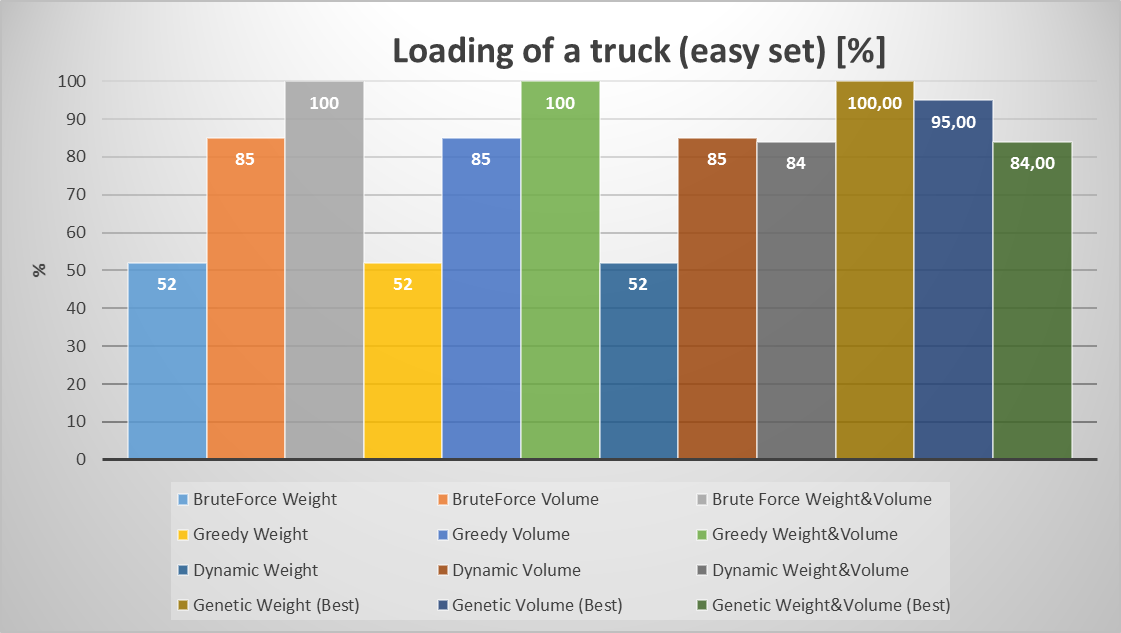
\includegraphics[width=\columnwidth]{image003.png}
  \caption{Percentage loading of a truck }
\end{figure}

\begin{figure}[H]
  \centering
  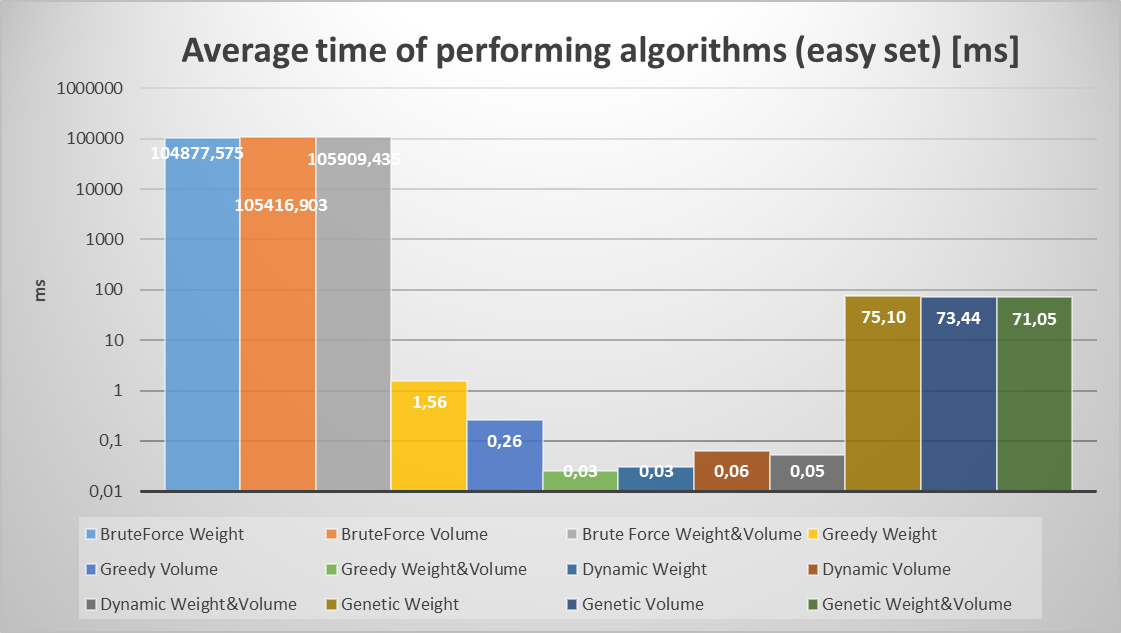
\includegraphics[width=\columnwidth]{image006.png}
  \caption{Average time of performing algorithms}
\end{figure}


As we can see on first diagram (Figure 1.) the best algorithm, as we take into account only weight or only volume of packages and truck, is Genetic Algorithm. In first case it found solution which loads a 100\% of maximum loading of a truck. In second case it obtained 95\%, which is very good result. However, if we want to consider both, the weight and the volume of packages and track at the same time, the best is Brute Force Algorithm and Greedy Algorithm. These algorithms obtained 100\% of loading of the truck.
If we take a look on the second diagram (Figure 2.) we can see that the fastest algorithm almost every time was Dynamic Programming. A little bit slower was Greedy Algorithm. As we were expecting the slowest algorithm was Brute Force Algorithm. Brute Force Algorithm tested with the smallest data set was executing almost 2 minutes while other algorithms was executing  less than 1 second and usually even much more faster.
The best (large fulfilment and high speed of execution) algorithm for the small data sets is Genetic Algorithm - if we look only on weight or only on volume, and Greedy Algorithm - if we want to consider these both things.\\

\item \textbf{Medium set}
\begin{figure}[H]
  \centering
  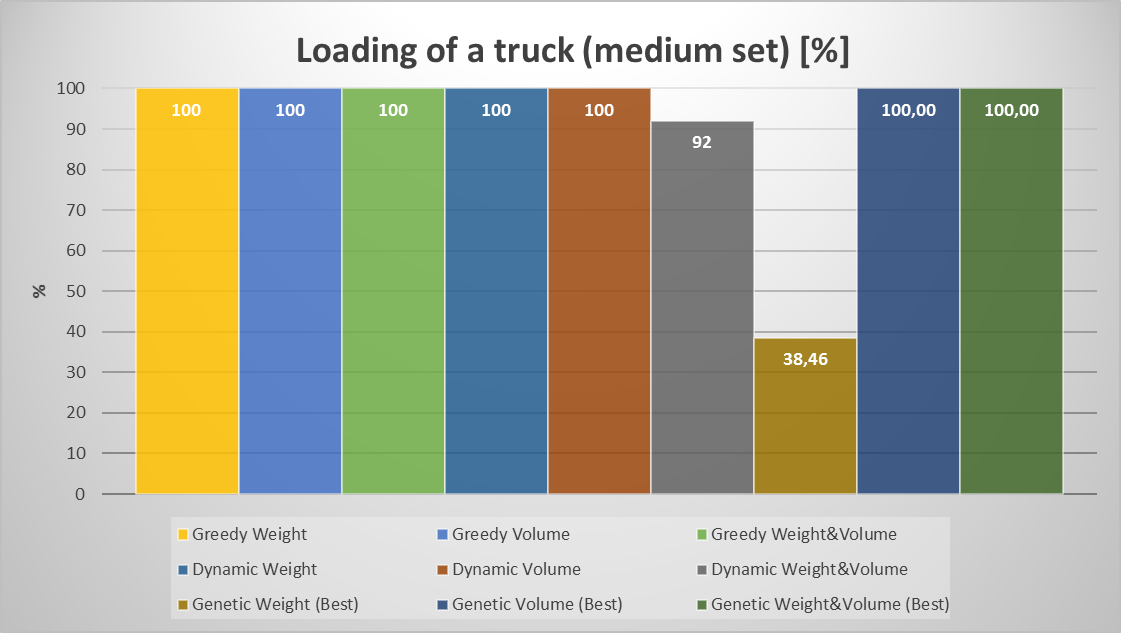
\includegraphics[width=\columnwidth]{image013.png}
  \caption{Percentage loading of a truck }
\end{figure}

\begin{figure}[H]
  \centering
  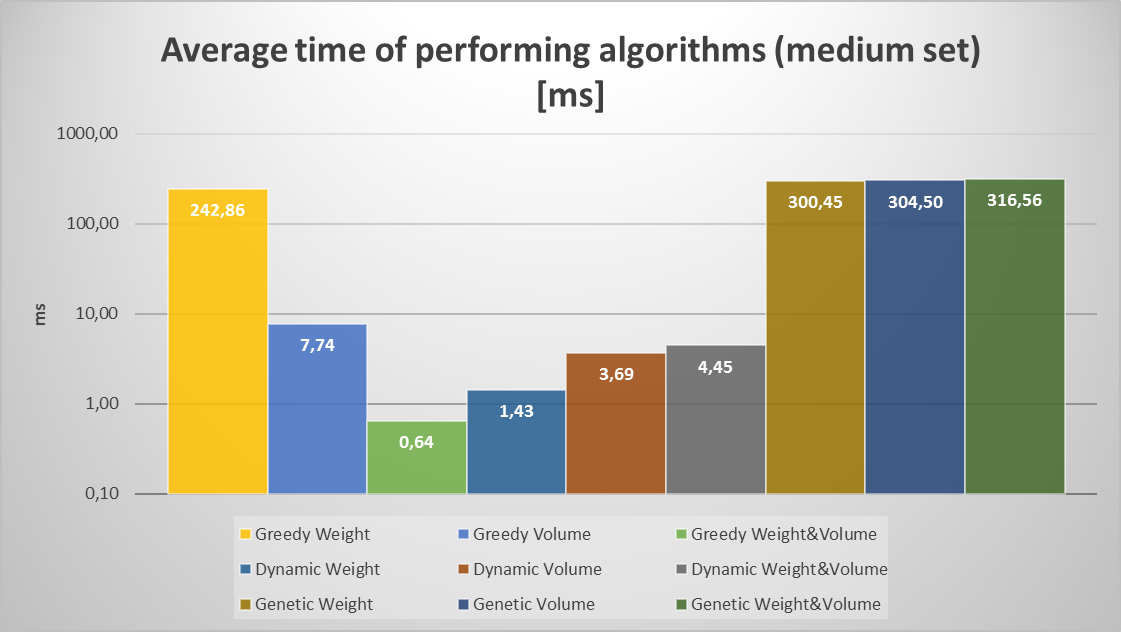
\includegraphics[width=\columnwidth]{image019.png}
  \caption{Average time of performing algorithms}
\end{figure}

As we can see on first diagram (Figure 3.) almost all algorithms give very well results. Only in two approach we can see anomaly: in Dynamic algorithm limited by both weight and volume and in Generic algorithm limited by weight.\\

Greedy algorithm limited by both weight and volume take the least time. Whereas 3. figure we agree that choosing this approach in this dataset could be the best solution.\\

\item \textbf{Hard set}

\begin{figure}[H]
  \centering
  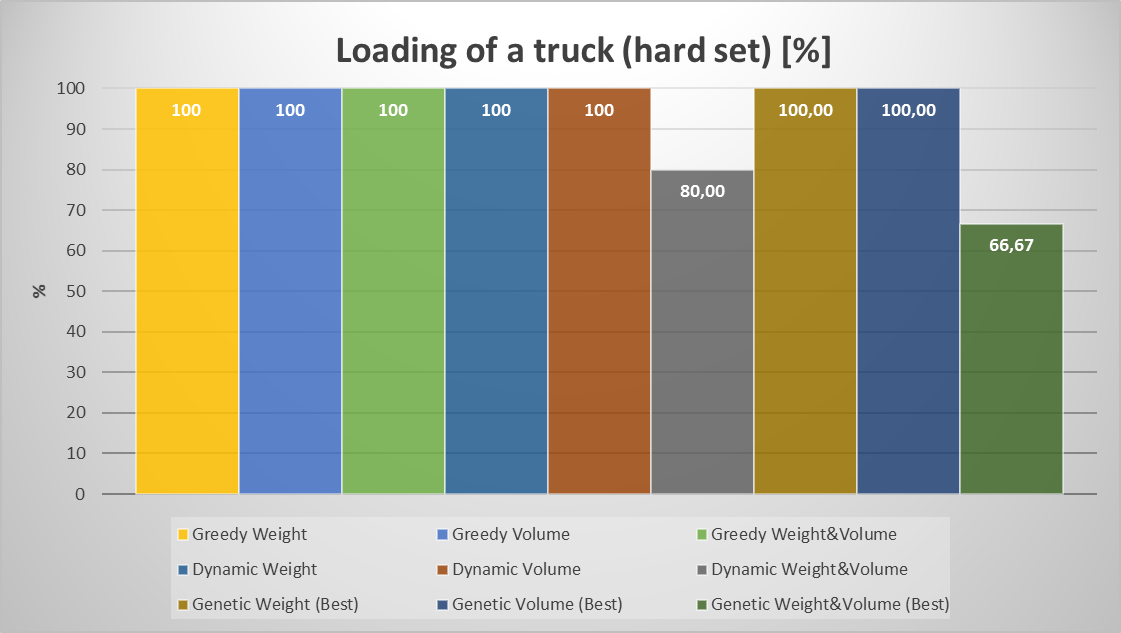
\includegraphics[width=\columnwidth]{image023.png}
  \caption{Percentage loading of a truck }
\end{figure}

\begin{figure}[H]
  \centering
  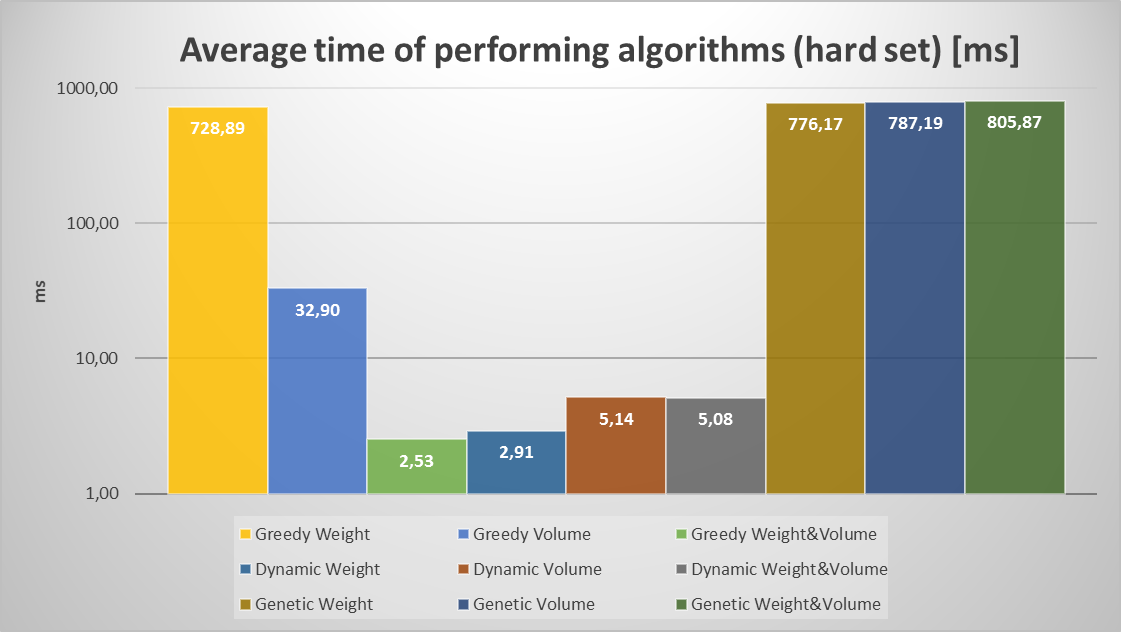
\includegraphics[width=\columnwidth]{image029.png}
  \caption{Average time of performing algorithms}
\end{figure}

As we can see on first diagram (Figure 5.) almost all algorithms give very well results. Again only in two approach we can see anomaly: in Dynamic algorithm limited by both weight and volume and in Generic algorithm limited by both weight and volume.\\

On the figure 5. we can see that Greedy algorithm limited by both weight and volume take the least time. Whereas 3. figure we agree that choosing this approach in this dataset could be the best solution.\\


\end{enumerate}





\section{Conclusion}
\begin{itemize}
\item Applying our programme in transport companies brings lots of benefits in example: saving time to load a truck or maximize cost of each loading;

\item After research each algorithm, we proved that the best one was "Greedy Algorithm", which we modified and it checked if each package was not too heavy (weight) or too big (volume). It was turning the best result of fulfilment a truck and also it was the fastest algorithm;

\item After research each algorithm, we proved that the best one was "Greedy Algorithm", which we modified and it checked if each package was not too heavy (weight) or too big (volume). It was turning the best result of fulfilment a truck and also it was the fastest algorithm;

\item The size of data set was mattered. The bigger set the longer was execution of each algorithm. We expected that kind of phenomenon;

\item It was impossible to test "Brute force Algorithm" using data set with lots of packages, because we didn't dispose so big computing power;

\end{itemize}




% use section* for acknowledgment
\ifCLASSOPTIONcompsoc
  % The Computer Society usually uses the plural form
  \section*{Acknowledgments}
\else
  % regular IEEE prefers the singular form
  \section*{Acknowledgment}
\fi

We would like to thank our professors: Leszek Koszalka and Wojciech Kmiecik for following us and support in hard moments. We also have to thank our two friends: Mariusz Lont and Marek Wosko, who helped us to invent a subject of our research (loading trucks). 




% trigger a \newpage just before the given reference
% number - used to balance the columns on the last page
% adjust value as needed - may need to be readjusted if
% the document is modified later
%\IEEEtriggeratref{8}
% The "triggered" command can be changed if desired:
%\IEEEtriggercmd{\enlargethispage{-5in}}

% references section

% can use a bibliography generated by BibTeX as a .bbl file
% BibTeX documentation can be easily obtained at:
% http://mirror.ctan.org/biblio/bibtex/contrib/doc/
% The IEEEtran BibTeX style support page is at:
% http://www.michaelshell.org/tex/ieeetran/bibtex/
%\bibliographystyle{IEEEtran}
% argument is your BibTeX string definitions and bibliography database(s)
%\bibliography{IEEEabrv,../bib/paper}
%
% <OR> manually copy in the resultant .bbl file
% set second argument of \begin to the number of references
% (used to reserve space for the reference number labels box)
\begin{thebibliography}{1}

\bibitem{IEEEhowto:kopka}
Thomas H. Cormen, Charles E. Leiserson, Ronald L. Rivest, Clifford Stein: \emph{Wprowadzenie do algorytmów.}\hskip 1em plus
0.5em minus 0.4em\relax Warszawa: Wydawnictwa Naukowo-Techniczne, 2003


\bibitem{IEEEhowto:kopka}
Michael R. Garey, David J. Johnson: \emph{Computers and intractability: a guide to the theory of NP-completeness.} \hskip 1em plus
0.5em minus 0.4em\relax San Francisco: W.H. Freeman, 1979


\bibitem{IEEEhowto:kopka}
Antoni Niederlański,\emph{Programowanie w logice z ograniczeniami}, wydanie 2 poprawione,\hskip 1em plus
0.5em minus 0.4em\relax Gliwce 2014


\bibitem{IEEEhowto:kopka}
Richard Neapolitan, \emph{Podstawy algorytmów z przykładami w C++},  \hskip 1em plus
0.5em minus 0.4em\relax Kumarss Naimipour, Helion 2004


\bibitem{IEEEhowto:kopka}
Jon Bentley, \emph{Perełki oprogramowania / Perełki programowania}, \hskip 1em plus
0.5em minus 0.4em\relax WNT/Helion, 2011

\bibitem{IEEEhowto:kopka}
Piotr Wroblewski, \emph{Algorytmy, struktury danych i techniki programowania. }, 3rd~ed.\hskip 1em plus
0.5em minus 0.4em\relax Gliwice, Helion, 2003.

\bibitem{IEEEhowto:kopka}
Wikipedia article on day 14-08-2016,
\\\texttt{https://en.wikipedia.org/wiki/Knapsack\_problem}

\bibitem{IEEEhowto:kopka}
Wikipedia article on day 14-08-2016,
\\\texttt{https://pl.wikipedia.org/wiki/Problem\_plecakowy}



\end{thebibliography}




% that's all folks
\end{document}


